\section{Implementing the linear algebra functions and the stencil operators [35 Points]}
After implementing the missing functions and the stencil kernel, given by the formula \ref{eq:stencil}, the serial code produces the output seen in Subfigure \ref{fig:serial}, which is approximately the same as the provided reference output in the project description.
\begin{equation} \label{eq:stencil}
f_{i, j}^k=\left[-(4+\alpha) s_{i, j}^k+s_{i-1, j}^k+s_{i+1, j}^k+s_{i, j-1}^k+s_{i, j+1}^k+\beta s_{i, j}^k\left(1-s_{i, j}^k\right)\right]+\alpha s_{i, j}^{k-1}
\end{equation}
Furthermore the resulting population concentration at final time is depicted in Subfigure \ref{fig:output_serial}.
\begin{figure}[H]
    \centering
    \begin{subfigure}[b]{0.6\textwidth}
        \centering
	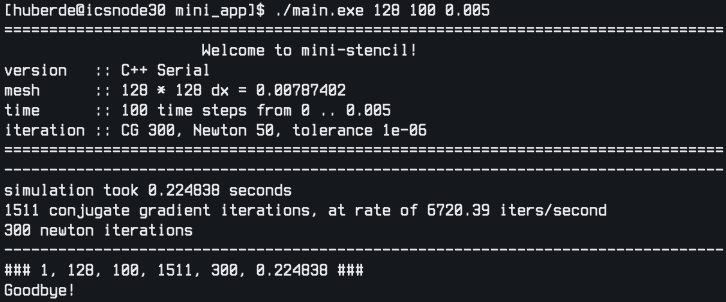
\includegraphics[width=\textwidth]{../media/serial_output.png}
	\caption{Output after implementing the linear algebra function and stencil operators.}
	\label{fig:serial}
    \end{subfigure}
    \hfill 
    \begin{subfigure}[b]{0.39\textwidth}
        \centering
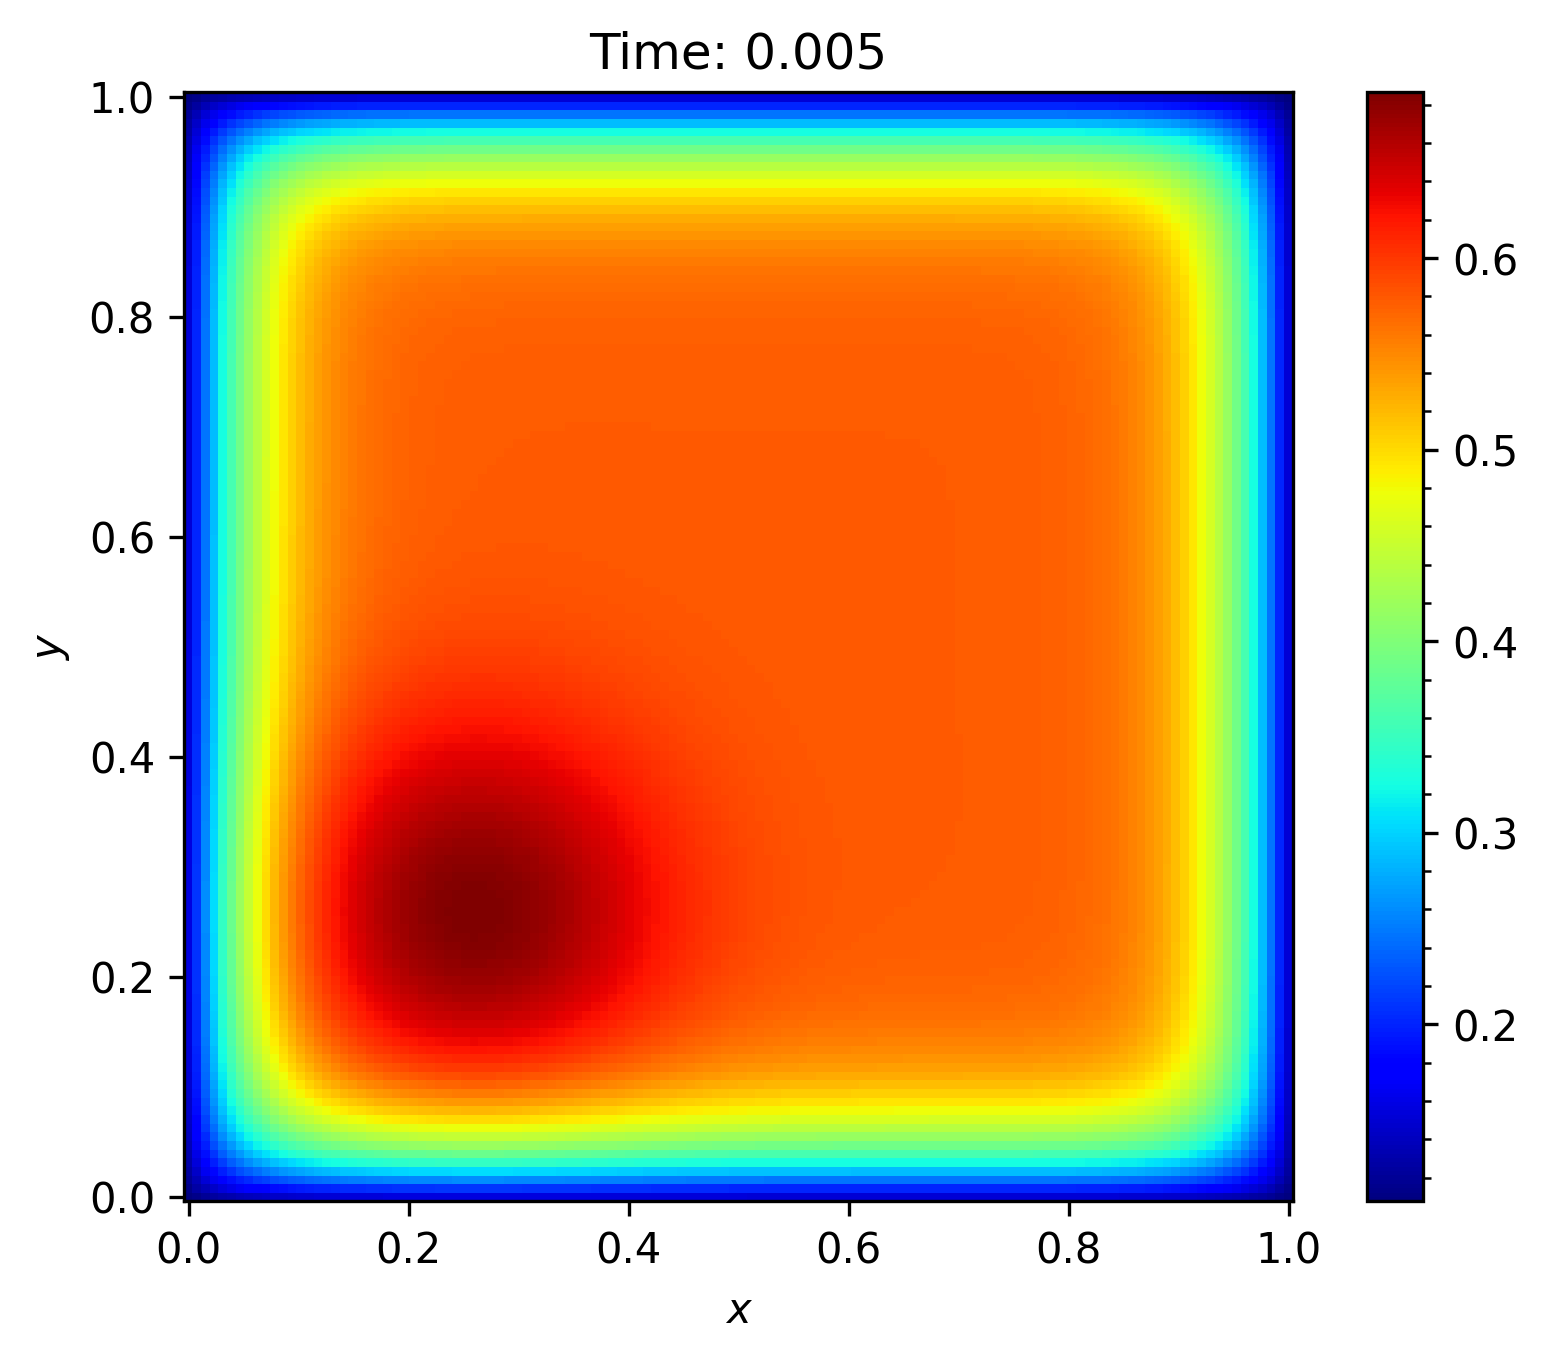
\includegraphics[width=\textwidth]{../media/output_serial.png}
	\caption{Population concentration at $t=0.005$.}
	\label{fig:output_serial}

    \end{subfigure}
    \caption{Results of the Mini App, when implemented in serial.}
    \label{fig:mini_app}
\end{figure}
